\documentclass[]{article}
\usepackage[a4paper, total={6in, 8in}]{geometry}
\usepackage{mathtools}
\usepackage{gensymb}
\usepackage{float}
\usepackage{graphicx}
\usepackage{multirow}
\usepackage{CJKutf8}
\usepackage{graphicx}
\usepackage{url}
\begin{CJK*}{UTF8}{bsmi} %gb
\title{CUDA Final Project Proposal}
\author{Wen-Liang, Huang 黃文亮}

\begin{document}
\maketitle

\section{2D \& 3D FFT with GPU}
We have already known the 1D fast Fourier transform\cite{FFT} with GPU in tutorial and the professor's code, and we also know that there are fundational library base on the Cooley-Tuckey\cite{Cooley-Tuckey} and Bluestein algorithms, and time result in GPU is better than CPU fast fourier transform. However; although I have read the three dimension FFT on GPU \cite{Keskin2017AnEP}, I still want to run the 2D FFT and 3D FFT in CPU and GPU, then compare the result of this two different types.

\begin{figure}[hbt!]
  \centering
  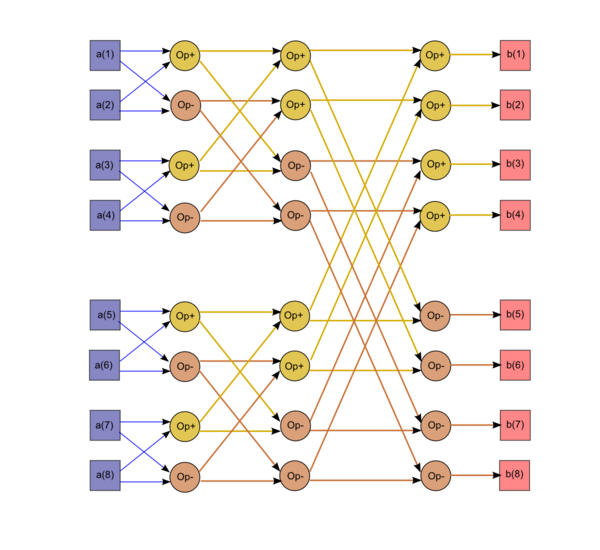
\includegraphics[height=7cm]{Cooley-Tukey_Fourier_Transform_algorithm}
  \caption{Simple Cooley-Tuckey Algorithm}
  \label{fig:mesh1}
\end{figure}

Next, I will quickly explain that how can we use the 2D and 3D fast Fourier transform.


\subsection{2D FFT}
In the 2D FFT, I have to check the 2D discrete Fourier transform and inverse discrete Fourier Transform
\begin{figure}[hbt!]
  \centering
  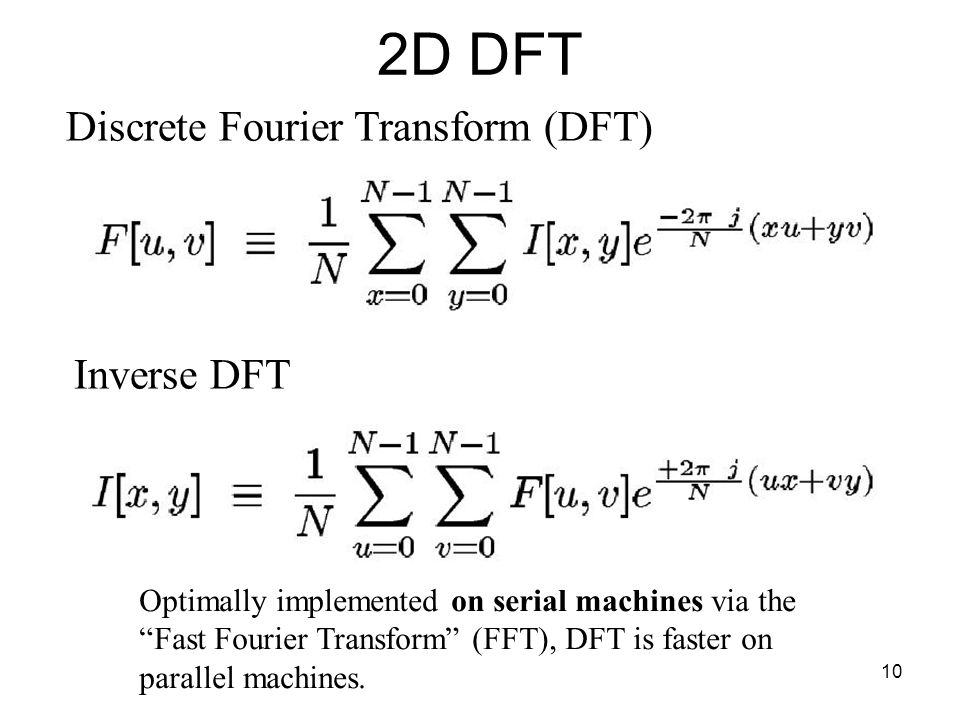
\includegraphics[width=6cm,height=4cm]{2D+DFT+Discrete+Fourier+Transform+(DFT)+Inverse+DFT}
  \caption{2D DFT}
\end{figure}
Actually, the 2D FFT is extended by 1D FFT.The concept is that I have to use the 1D FFT in each column at first, then using the transform result to put them into each row.
\subsection{3D FFT}
There is no suitable 3D FFT coding, but I think it just add another one dimension from 2D FFT, but remember, I have to run each column, then use the result of each column to put into each row, then use the result of each row to put into the next dimension.
\section{Expected Result}
There are two temporary expected result in my proposal
\subsection{Run time in 2D \& 3D FFT }
Compared the runtime of 2D and 3D FFT with GPU to the runtime of 2D and 3D FFT with CPU, I expect that the run time of the previous one is less than the later one.
\subsection{Other Application with FFT}
Using the library of FFT in Nvidia and implement some social application.
\begin{figure}[hbt!]
  \centering
  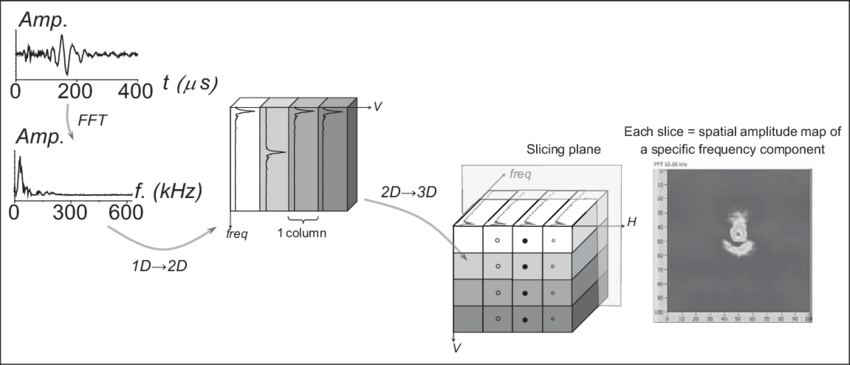
\includegraphics[width=10cm,height=5cm]{Ultrasonic-spectral-imaging-algorithm-ACT-air-coupled-transducer-FFT-fast-Fourier}
  \caption{FFT of 1D to 2D to 3D}
  \label{fig:mesh1}
\end{figure}
\medskip
%\begin{thebibliography}{10}

%\bibitem{FFT}
%Fast Fourier Transform
%\\\texttt{https://en.wikipedia.org/wiki/Fast\char`_Fourier\char`_transform}
%\bibitem{Cooley-Tuckey}
%Cooley-Tuckey algorithm in Fast Fourier Transform,
%\\\texttt{https://en.wikipedia.org/wiki/Cooley-Tukey\char`_FFT\char`_algorithm}
\bibliographystyle{unsrt}
\bibliography{sample}
%\end{thebibliography}

\end{CJK*}
\end{document}
